\documentclass[10pt,a4paper]{article}
\usepackage[utf8]{inputenc}
\usepackage[italian]{babel}
\usepackage{amsmath}

\usepackage{amsfonts}
\usepackage{amssymb}
\usepackage{graphicx}
\usepackage[left=2cm,right=2cm,top=2cm,bottom=2cm]{geometry}
\newcommand{\rem}[1]{[\emph{#1}]}
\newcommand{\exn}{\phantom{xxx}}
\renewcommand{\thesubsection}{\thesection.\alph{subsection}}  %% use 1.a numbering

\author{Gruppo 1G.BN \\ Massimo Bilancioni, Alessandro Foligno, Giuseppe Zanichelli }
\title{Es05B: Circuiti lineari con Amplificatori Operazionali}
\begin{document}
	\date{8 novembre 2018}
	\maketitle
	
	
	\section*{Scopo dell' esperienza}
	Misurare le caratteristiche di circuiti lineari realizzati con un op-amp TL081 alimentati tra +15 V e -15 V.
	
	\section{Amplificatore invertente}
	Si vuole realizzare un amplificatore invertente con un'~impedenza di ingresso superiore a 1 
	k$\Omega$ e con un amplificazione a centro banda di 10.
	
	\subsection{Scelta dei componenti}
	
	Si monta il circuito secondo lo schema mostrato in figura, utilizzando la barra di 
	distribuzione verde per la tensione negativa, quella rosso per la tensione positiva, e quella nera per 
	la massa.
	
	\rem{Indicare i criteri di scelta delle resistenze ed i valori desiderati}\\

	
	Le resistenze selezionate hanno i seguenti valori, misurati con il multimetro digitale, con il corrispondente valore atteso 
	del guadagno in tensione dell'~amplificatore.
	\[
	R_1 = ( 1.466 \pm 0.012) \,\mathrm{k}\Omega, \quad 
	R_2 = (15.24  \pm 0.12) \,\mathrm{k}\Omega, \quad 
	A_{exp} = ( -10.39 \pm 0.11)
	\]
	
	\subsection{Montaggio circuito}
	Il circuito è stato montato nella basetta come riportato in figura.
	%%%%%%%%%%%%%%%%%%%%%%%%%%%%%%%%%%%%%%%%%%%%%%%%%%%%%%
	\subsection{Linearit\`a e misura del guadagno}
	Si fissa la frequenza del segnale ad $f_{in} = (2.597 \pm 0.011)$ kHz e si invia all'~ingresso dell'~amplificatore.	L'uscita dell'~amplificatore \`e mostrata qualitativativamente in Fig. \ref{fig:oscinv} per due 
	differenti ampiezze di $V_{in}$ (circa $1.26$~Vpp e $7.20$~Vpp). 
	Nel primo caso l'~OpAmp si comporta in modo lineare mentre nel secondo caso si osserva clipping. Il datasheet riporta uno Slew rate di $13 V/\mu s$ che è quindi trascurabile a questa frequenza .
	%
	\begin{figure}[h]
		\begin{center}
		
			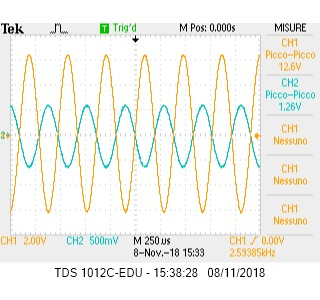
\includegraphics[scale=0.7]{foto1.jpg}
			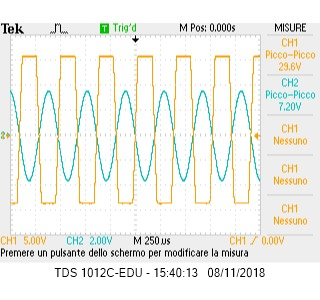
\includegraphics[scale=0.7]{foto2.jpg}
			\caption{screenshot dei segnali con e senza clipping}
			%\includegraphics[0.45\textwidth]{}
		\end{center}
		\caption{\small Ingresso (in alto) ed uscita (in basso) di un amplificatore invertente con OpAmp, in 
			zona lineare (a sinistra) e non (a destra)}
		\label{fig:oscinv}
	\end{figure}
	%
	
	Variando l'~ampiezza di $V_{in}$ si misura $V_{out}$ ed il relativo guadagno $A_V=V_{out}/V_{in}$ riportando i dati ottenuti in tabella~\ref{tab:guadagno} 
	e mostrandone un grafico in Fig. \ref{fig:lin}. 
	
	\begin{table}[h]
		\caption{$V_{out}$ in funzione di $V_{in}$ e relativo rapporto.}
		\label{tab:guadagno}
		\begin{center}
			\begin{tabular}{|c|c|c|}
				\hline
				$V_{in}$ (V) & $V_{out}$ (V)  & $A_V$ \\
				\hline
				\hline
				$\exn \pm \exn $ & $\exn \pm \exn $ & $\exn \pm \exn$ \\
				\hline
				$\exn \pm \exn $ & $\exn \pm \exn $ & $\exn \pm \exn $ \\
				\hline
				$\exn \pm \exn $ & $\exn \pm \exn $ & $\exn \pm \exn $ \\
				\hline
				$\exn \pm \exn $ & $\exn \pm \exn $ & $\exn \pm \exn $ \\
				\hline
				$\exn \pm \exn $ & $\exn \pm \exn $ & $\exn \pm \exn $ \\
				\hline
			\end{tabular}
		\end{center}
	\end{table}
	\begin{figure}
			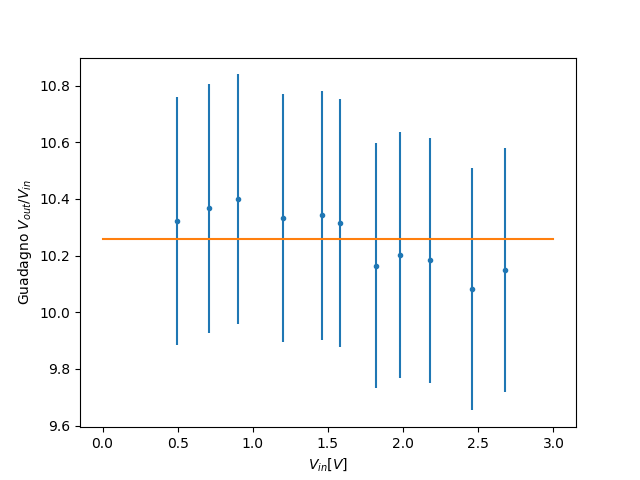
\includegraphics[scale=0.5]{fit.png}
	\end{figure}
	\rem{Indicare in che modo si fa il fit, se sulla retta $V_{out}$ vs. $V_{in}$ oppure sui valori di $A_V$   }
	
	Si determina il guadagno mediante fit dei dati ottenuti:
	\[
	A_{best} = \exn \pm \exn \quad  \chi^2 = \exn
	\]
	\begin{figure}[t]
		\begin{center}
			\framebox(200,200){Inserire grafico con di $V_{out}$ e $V_{in}$}
			%\includegraphics[0.8\textwidth]{}
		\end{center}
		\caption{\small Linearit\`a dell'~amplificatore invertente}
		\label{fig:lin}
	\end{figure}
	%
	
	\rem{Fino a quale tensione il circuito si comporta linearmente? Provare (facoltativamente) a ridurre la 
		tensione di alimentazione dell'~integrato ed a verificarne la correlazione con la tensione di 
		\emph{clipping} dell'~uscita. Commentare quanto osservato }
	
	%%%%%%%%%%%%%%%%%%
	%
	\section{Risposta in frequenza e \emph{slew rate}}
	\subsection{Risposta in frequenza del circuito}
	Non siamo riusciti a vedere la frequenza di taglio inferiore, che tuttavia deve essere   $\l 10\mathrm{Hz}$ visto che per questa frequenza  non si ha una sensibile diminuzione del guadagno.

 Per la frequenza di taglio superiore abbiamo campionato il guadagno per frequenze tra $1\mathrm{kHz}$ e $ 1\mathrm{MHz}.$
Abbiamo abbassato $V_{in}$ per alte frequenze per evitare per evitare  possibili Slew Rate.

La frequenza di taglio è stata ricavata come l'intersezione delle due rette fittate rispettivamente a bassa e ad alta frequenza.
(Figura 4)


	
	\[
	f_H = (167.7 \pm \exn \;)\,\mathrm{kHz}
	\]
	\begin{table}[h]
		\caption{\small Guadagno dell'~amplificatore invertente in funzione della frequenza.}
		\label{tab:bodeinv}
		\begin{center}
			\begin{tabular}{|c|c|c|c|}	\hline
				$f_{in}$ (kHz) & $V_{in}$ (V) & $V_{out}$ (V) & $A$ (dB) \\
				\hline
				$\exn0.753 \pm0.015 \exn $ & $\exn1.02 \pm 0.03\exn$ & $\exn10.4 \pm 0.3 \exn $ & $\exn 20.2\pm 0.26\exn $\\
				\hline
				$\exn 1.76\pm 0.04\exn $ & $\exn1.03\pm 0.03\exn$ & $\exn 10.5\pm 0.3\exn $ & $\exn 20.2\pm0.26 \exn $\\
\hline


				\hline
				$\exn 2.90\pm0.06 \exn $ & $\exn1.03 \pm 0.03\exn$ & $\exn 10.5\pm 0.3 \exn $ & $\exn 20.2\pm0.26 \exn $\\
				\hline
				$\exn 6.22\pm0.12 \exn $ & $\exn1.05 \pm0.03 \exn $& $\exn 10.7\pm 0.3 \exn $ & $\exn 20.2\pm0.26 \exn $\\
				\hline
				$\exn 12.2\pm 0.2\exn $  & $\exn1.06 \pm0.03 \exn$& $\exn 10.7\pm 0.3 \exn $ & $\exn 20.1\pm0.26 \exn $\\
				\hline
				$\exn22.5 \pm 0.4\exn $ & $\exn1.05\pm0.03 \exn $& $\exn 10.6\pm 0.3 \exn $ & $\exn20.1\pm0.26 \exn $\\
				\hline
				$\exn44.9 \pm0.9 \exn $ & $\exn1.05 \pm 0.03\exn$ & $\exn10.5 \pm 0.3 \exn $ & $\exn 20.0\pm0.26 \exn $\\
				\hline
				$\exn 86.7\pm1.7 \exn $ & $\exn1.06 \pm 0.03\exn$ & $\exn9.92 \pm 0.3 \exn $ & $\exn 19.4\pm0.26 \exn $\\
				\hline
				$\exn 166\pm 3\exn $  & $\exn1.06 \pm 0.03\exn$& $\exn8.48 \pm 0.3 \exn $ & $\exn 18.1 \pm0.26 \exn $\\
  \hline
				$\exn212\pm  4\exn $ & $\exn 0.688\pm 0.02 \exn$ & $\exn4.96 \pm 0.15\exn $ & $\exn 17.2\pm 0.26 \exn $\\

\hline
				$\exn251 \pm 5 \exn $  & $\exn0.680 \pm 0.02\exn$& $\exn4.44 \pm0.14 \exn $ & $\exn 16.3\pm 0.26 \exn $\\
				\hline
				$\exn 350\pm 7\exn $  & $\exn0.776 \pm 0.02\exn$& $\exn 4.02\pm 0.13\exn $ & $\exn14.3\pm0.26 \exn $\\
				\hline
				$\exn 435\pm 9 \exn $ & $\exn0.688\pm0.02 \exn$ & $\exn 3.00\pm 0.09 \exn $ & $\exn 12.8\pm0.26 \exn $\\
				\hline
				$\exn555 \pm 10  \exn $ & $\exn0.696 \pm0.02 \exn$ & $\exn2.44 \pm 0.08\exn $ & $\exn 10.9 \pm0.26 \exn $\\
				\hline
				$\exn 729 \pm  14\exn $ & $\exn0.784\pm0.02 \exn$ & $\exn 2.22\pm 0.07\exn $ & $\exn 9.04 \pm0.26 \exn $\\
				\hline
				$\exn 1220\pm 24\exn $  & $\exn 0.800 \pm 0.03\exn$& $\exn 1.38\pm 0.05\exn $ & $\exn 4.74\pm0.26 \exn $\\
				

				\hline
			\end{tabular}
		\end{center}
	\end{table} 
	
	
	
	\begin{figure}[h]
		\begin{center}
			
			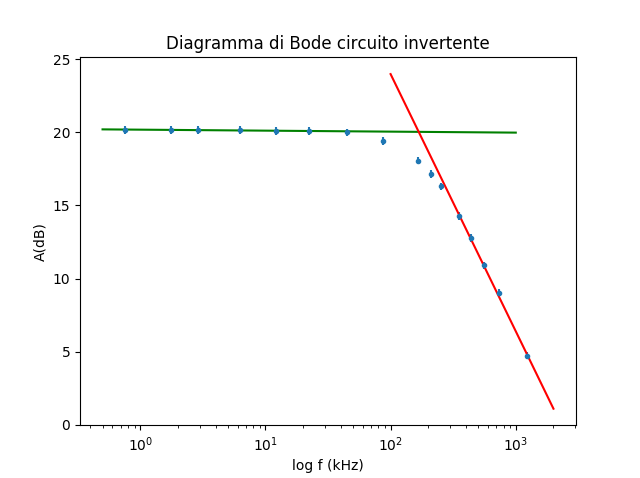
\includegraphics[width=0.7\textwidth]{bodeInvertente}
			\caption{\small Plot di Bode in ampiezza per l'~amplificatore invertente.}
			\label{fig:bodeinv}
		\end{center}
	\end{figure}
	%
	\subsection{Misura dello \emph{slew-rate}}
	Si misura direttamente lo \emph{slew-rate} dell'op-amp inviando in ingresso un'~onda quadra 
	di frequenza intorno ai $\sim 0.9$~kHz e di ampiezza $2.08$~V. Si ottiene:
	\[
	SR_\mathrm{misurato} = (12.5 \pm 0.5 )\,\mathrm{V/\mu s} \quad \mathrm{valore \; tipico}\, (13 )\,\mathrm{V/\mu s}\
	\]
Abbiamo misurato la  pendenza massima del segnale $V_{out}$, che si trova proprio  in corrispondenza dell' inizio dell'onda quadra, subito dopo la pendenza diminuisce di circa 0.5 $ \mathrm{V/\mu s}$

\begin{figure}[h]
		\begin{center}
			
			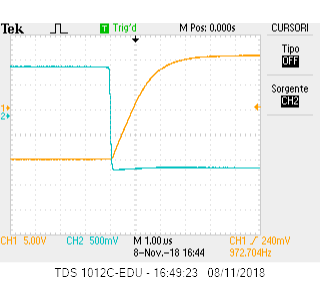
\includegraphics[width=0.7\textwidth]{slewrate}
			\caption{\small Segnale onda quadra (azzurro) e $V_{in}$ (arancio)}
			\label{fig:Slew  Rate}
		\end{center}
	\end{figure}

	\section{Circuito integratore}
	Si monta il circuito integratore con i seguenti valori  dei componenti indicati: 
	\[
	R_1 = (0.997 \pm 0.008 \;) \,\mathrm{k}\Omega, \:\:\;\:\exn 
	R_2 = (9.92 \pm 0.08 \;) \,\mathrm{k}\Omega, \:\:\;\:\exn 
	C = (50.4 \pm 2.3 \;\;)\,\mathrm{nF}
	\]
	
	\subsection{Risposta in frequenza}
	
	Si invia un'~onda sinusoidale e si misura la risposta in frequenza dell'~amplificazione e della fase riportandoli 
	nella tabella \ref{tab:bodeinte} e in un diagramma di Bode in Fig. \ref{fig:bodeinte}. 
	\[
	V_{in} = (\exn \pm \exn )\,\mathrm{V}
	\]
	\rem{La fase pu\'o essere indicata in gradi, radianti, oppure come frazione $\phi/2\pi$}
	%
	\begin{table}[h]
		\caption{Guadagno e fase dell'~integratore invertente in funzione della frequenza.}
		\label{tab:bodeinte}
		\begin{center}
			\begin{tabular}{|c|c|c|c|c|}
				\hline
				$f_{in}$ (kHz) & $V_{out}$ (V) & $A$ (dB) & $\Delta t (\mu s)$ & $\phi$ \\
				\hline
				$\exn \pm \exn $ & $\exn \pm \exn $ & $\exn \pm \exn $ & $\exn \pm \exn $ & $\exn \pm \exn $ \\
				\hline
				$\exn \pm \exn $ & $\exn \pm \exn $ & $\exn \pm \exn $ & $\exn \pm \exn $ & $\exn \pm \exn $ \\
				\hline
				$\exn \pm \exn $ & $\exn \pm \exn $ & $\exn \pm \exn $ & $\exn \pm \exn $ & $\exn \pm \exn $ \\
				\hline
				$\exn \pm \exn $ & $\exn \pm \exn $ & $\exn \pm \exn $ & $\exn \pm \exn $ & $\exn \pm \exn $ \\
				\hline
				$\exn \pm \exn $ & $\exn \pm \exn $ & $\exn \pm \exn $ & $\exn \pm \exn $ & $\exn \pm \exn $ \\
				\hline
				$\exn \pm \exn $ & $\exn \pm \exn $ & $\exn \pm \exn $ & $\exn \pm \exn $ & $\exn \pm \exn $ \\
				\hline
				$\exn \pm \exn $ & $\exn \pm \exn $ & $\exn \pm \exn $ & $\exn \pm \exn $ & $\exn \pm \exn $ \\
				\hline
			\end{tabular}
		\end{center}
	\end{table} 
	%
	\begin{figure}[htb]
		\begin{center}
			\framebox(200,200){Inserire plot di Bode in ampiezza}
			\framebox(200,200){Analogo in fase}
			%\includegraphics[0.45\textwidth]{}
			%\includegraphics[0.45\textwidth]{}
		\end{center}
		\caption{\small Plot di Bode in ampiezza (a sinistra) e fase (a destra) per il circuito integratore.}
		\label{fig:bodeinte}
	\end{figure}
	%
	
	Si ricava una stima delle caratteristiche principali dell'andamento (guadagno a bassa frequenza, frequenza di taglio, e pendenza ad alta frequenza)
	e si confrontano con quanto atteso. Non si effettua la stima degli errori, trattandosi di misure qualitative.
	
	\rem{Indicare brevemente come sono stati ottenuti i valori attesi}
	
	\begin{align*}
	A_M &= (\exn )\,\mathrm{dB} & \mathrm{atteso} &:\,(\exn  )\, \mathrm{dB}  \\
	f_H &= (\exn )\,\mathrm{Hz} & \mathrm{atteso} &:\,(\exn  )\, \mathrm{Hz} \\
	{\mathrm{d}A_V}/{\mathrm{d}f} &= (\exn )\,\mathrm{dB/decade} & \mathrm{atteso} &:\,(\exn  )\, \mathrm{dB/decade}  \\
	\end{align*}
	
	
	%
	\subsection*{Risposta ad un'~onda quadra}
	Si invia all'~ingresso un'~onda quadra di frequenza $\sim xxx\,kHz$ e ampiezza $\sim xxx\,V$.
	Si riporta in Fig. \ref{fig:oscinte} le forme d'~onda acquisite all'~oscillografo per l'~ingresso
	e l'~uscita. 
	
	\rem{Commentare se che il circuito si comporta come un integratore.}
	%
	\begin{figure}[htb]
		\begin{center}
			\framebox(200,200){Inserire screenshot oscillografo per integratore}
			%\includegraphics[0.45\textwidth]{}
		\end{center}
		\caption{\small Ingresso (in alto) ed uscita (in basso) del circuito integratore per un'~onda quadra.}
		\label{fig:oscinte}
	\end{figure}
	%
	
	Si misura l'~ampiezza dell'~onda  in uscita e si confronta il valore atteso.
	
	\rem{Indicare brevemente come sono stati ottenuti i valori attesi}
	\begin{align*}
	V_{out} &= (\exn )\,\mathrm{V} & \mathrm{atteso} &:\,(\exn  )\, \mathrm{V}  \\
	\end{align*}
	
	\rem{Inserire commento sulla dipendenza dell'~uscita dalla frequenza.}
	%
	
	\subsection{Discussione}
	
	\rem{Inserire commenti su quanto osservato ed eventuali deviazioni. 
		In particolare: attenuazione ad alte frequenze, dipendenza della fase dalla frequenza, funzione di $R_2$. }
	
	%%%%%%%%%%%%%%%%%%%%%%%%
	
\end{document}          
